\documentclass[border=10pt]{standalone}
\usepackage{tikz}
\usepackage{xcolor}
\usetikzlibrary{arrows.meta,positioning,calc,fit,backgrounds}

% --- wire colors (matching real Dupont colors) ---
\definecolor{wireRed}{RGB}{220,40,40}
\definecolor{wireOrange}{RGB}{240,140,0}
\definecolor{wireYellow}{RGB}{220,190,0}
\definecolor{wireGreen}{RGB}{50,160,60}
\definecolor{wireBlue}{RGB}{40,90,210}
\definecolor{wirePurple}{RGB}{140,50,180}
\definecolor{wireBrown}{RGB}{120,75,40}
\definecolor{wireWhite}{RGB}{220,220,220}
\definecolor{wireGray}{RGB}{130,130,130}
\definecolor{wireBlack}{RGB}{30,30,30}

\begin{document}
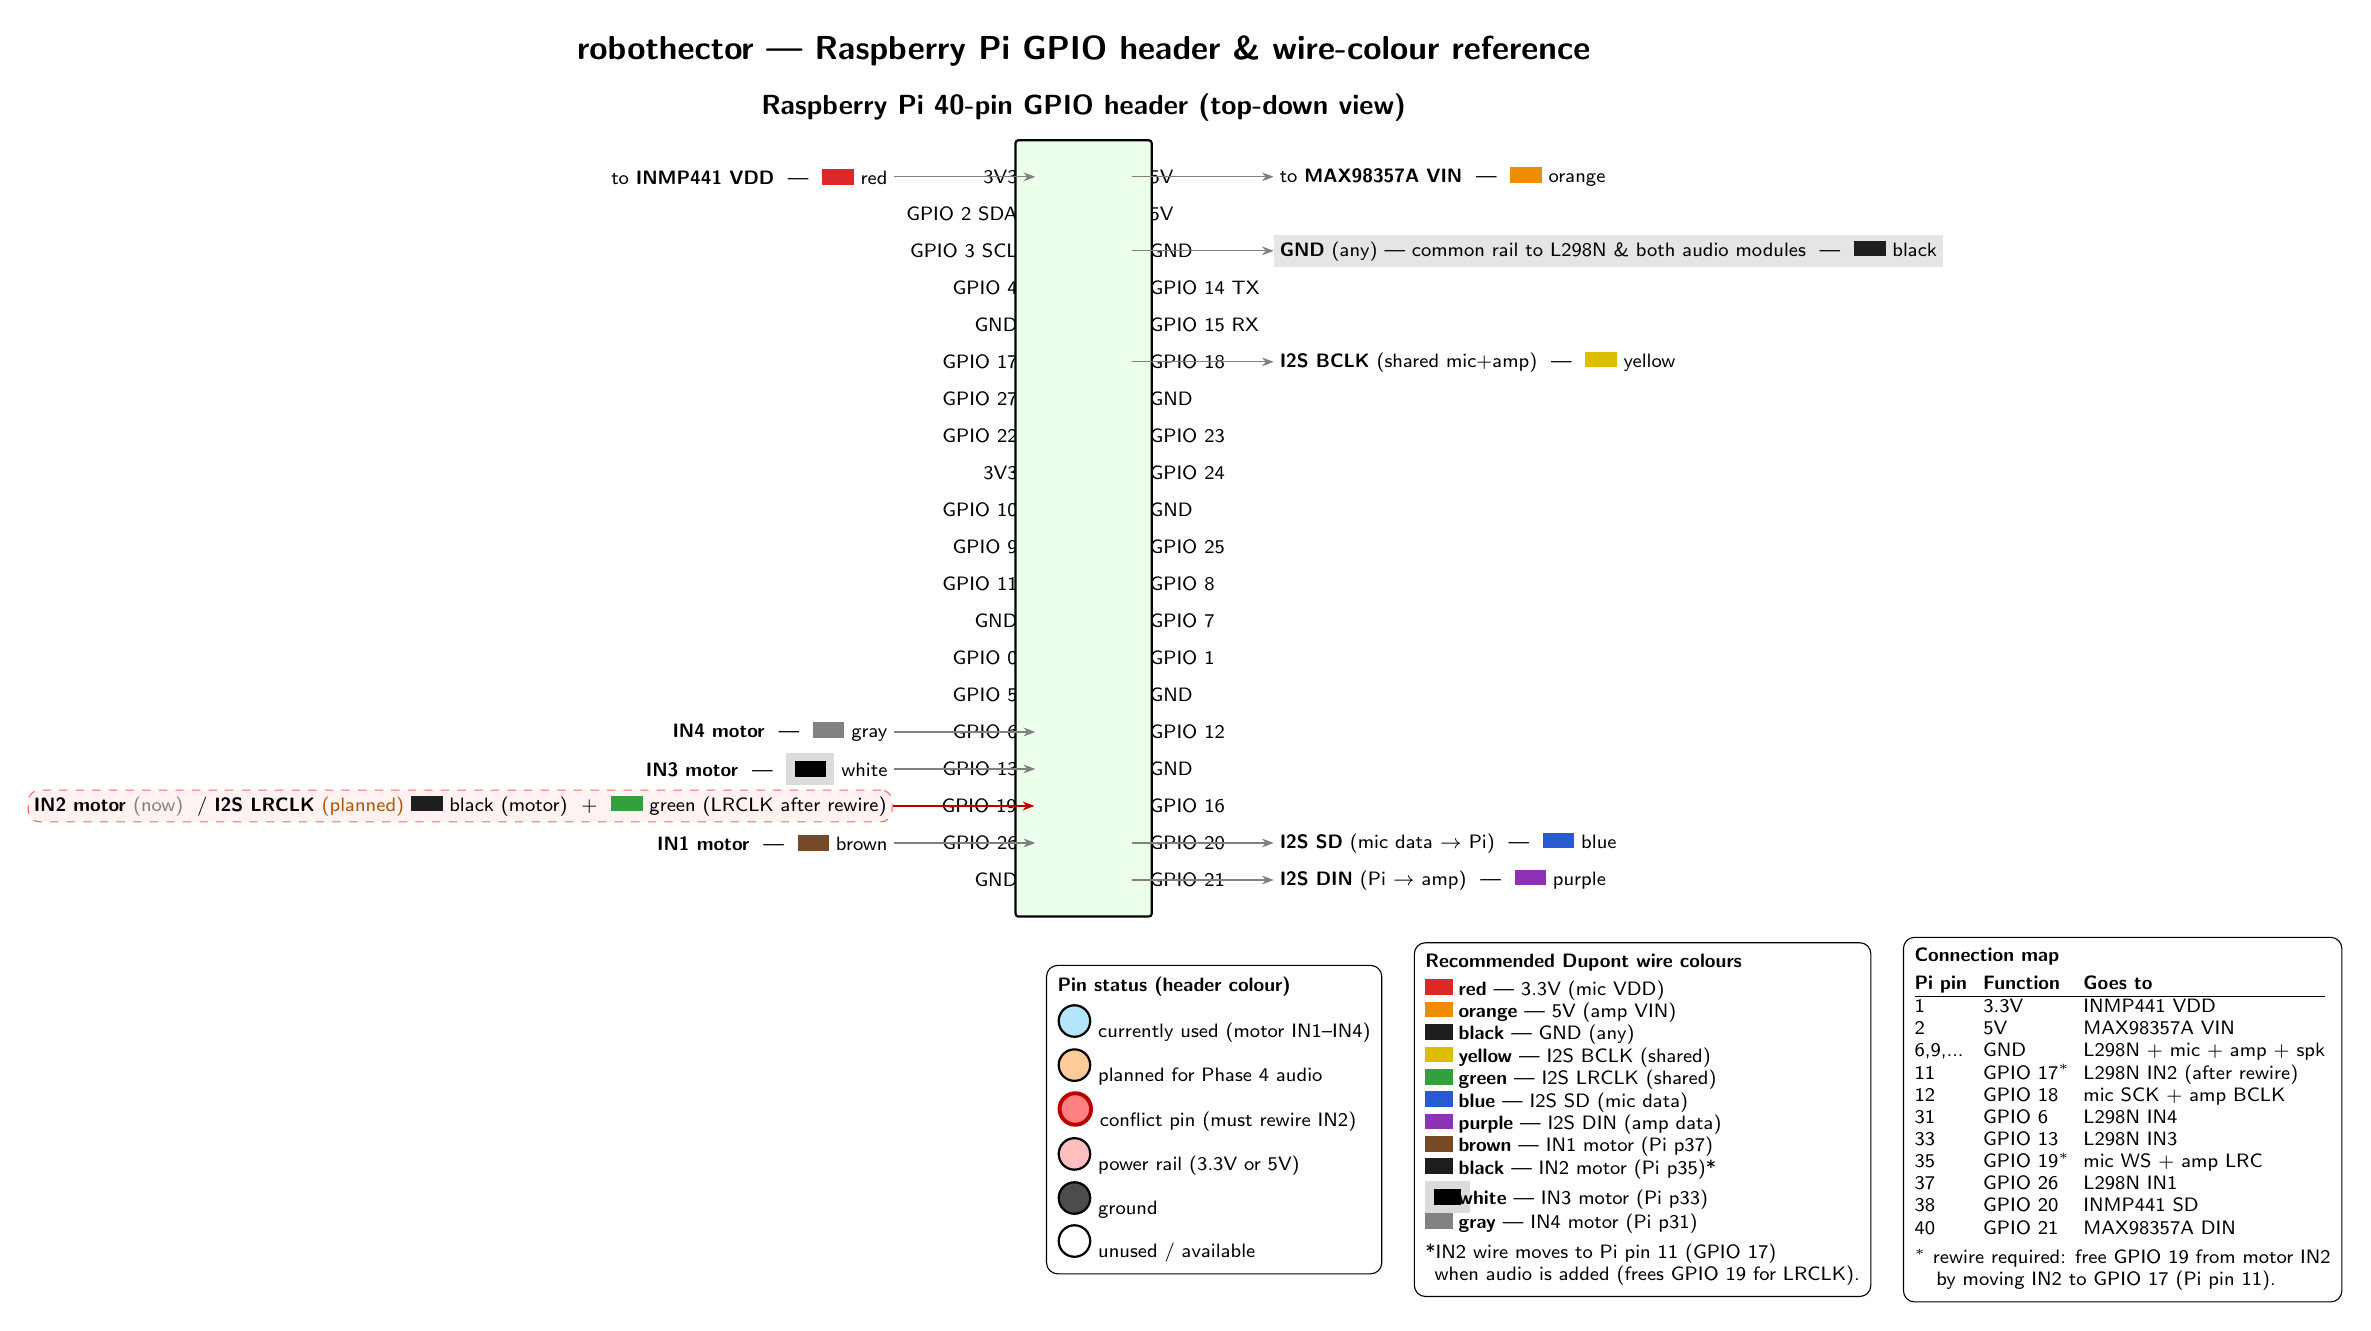
\begin{tikzpicture}[
    font=\sffamily\footnotesize,
    pin/.style={draw, thick, circle, minimum size=4mm, inner sep=0pt, fill=white,
                font=\sffamily\scriptsize\bfseries},
    pinUsed/.style={pin, fill=cyan!30},
    pinPlanned/.style={pin, fill=orange!40},
    pinPower/.style={pin, fill=red!25},
    pinGnd/.style={pin, fill=black!70, text=white},
    pinFree/.style={pin, fill=white},
    pinConflict/.style={pin, fill=red!50, draw=red!75!black, line width=0.5mm},
    fnL/.style={anchor=east, font=\sffamily\scriptsize},
    fnR/.style={anchor=west, font=\sffamily\scriptsize},
    pinNum/.style={font=\sffamily\tiny, text=black!60},
    callout/.style={anchor=west, font=\sffamily\scriptsize, inner sep=2pt},
    swatch/.style={draw=black!40, line width=0.3pt, minimum size=3mm,
                   inner sep=0pt, font=\sffamily\tiny},
  ]

  %================================================================
  % 40-pin header — two columns, 20 rows
  %================================================================
  \def\rowstep{4.7mm}
  \def\colgap{8mm}

  % helper coordinates
  \coordinate (origin) at (0,0);

  % Pin definitions: row, leftStyle, leftFn, leftPinNum, rightStyle, rightFn, rightPinNum
  % rows count from 1 (top) to 20 (bottom)
  \foreach \r/\lstyle/\lfn/\lpin/\rstyle/\rfn/\rpin in {%
     1/pinPower/3V3/1     /pinPower/5V/2,
     2/pinFree/GPIO 2 SDA/3 /pinPower/5V/4,
     3/pinFree/GPIO 3 SCL/5 /pinGnd/GND/6,
     4/pinFree/GPIO 4/7   /pinFree/GPIO 14 TX/8,
     5/pinGnd/GND/9       /pinFree/GPIO 15 RX/10,
     6/pinFree/GPIO 17/11 /pinPlanned/GPIO 18/12,
     7/pinFree/GPIO 27/13 /pinGnd/GND/14,
     8/pinFree/GPIO 22/15 /pinFree/GPIO 23/16,
     9/pinPower/3V3/17    /pinFree/GPIO 24/18,
    10/pinFree/GPIO 10/19 /pinGnd/GND/20,
    11/pinFree/GPIO 9/21  /pinFree/GPIO 25/22,
    12/pinFree/GPIO 11/23 /pinFree/GPIO 8/24,
    13/pinGnd/GND/25      /pinFree/GPIO 7/26,
    14/pinFree/GPIO 0/27  /pinFree/GPIO 1/28,
    15/pinFree/GPIO 5/29  /pinGnd/GND/30,
    16/pinUsed/GPIO 6/31  /pinFree/GPIO 12/32,
    17/pinUsed/GPIO 13/33 /pinGnd/GND/34,
    18/pinConflict/GPIO 19/35 /pinFree/GPIO 16/36,
    19/pinUsed/GPIO 26/37 /pinPlanned/GPIO 20/38,
    20/pinGnd/GND/39      /pinPlanned/GPIO 21/40%
  }{%
     % left pin
     \node[\lstyle] (Lp\r) at (0, -\r*\rowstep) {\lpin};
     \node[fnL] at ([xshift=-1mm]Lp\r.west) {\lfn};
     % right pin
     \node[\rstyle] (Rp\r) at (\colgap, -\r*\rowstep) {\rpin};
     \node[fnR] at ([xshift=1mm]Rp\r.east) {\rfn};
  }

  % header outline
  \node[draw, thick, rounded corners=1pt, fit=(Lp1)(Rp20),
        inner sep=2.5mm, fill=green!8, on background layer] (header) {};

  \node[font=\sffamily\bfseries, above=1mm of header.north]
        {Raspberry Pi 40-pin GPIO header (top-down view)};

  %================================================================
  % CALLOUTS — one per used/planned pin, with wire colour
  %================================================================
  % left side callouts (for left column pins): place to the LEFT of the function
  % right side callouts: place to the RIGHT of the function
  % stagger horizontally so they don't overlap

  \def\leftPad{18mm}   % distance from header centre to callout start (left side)
  \def\rightPad{18mm}

  % --- LEFT column callouts ---
  % pin 1 — 3V3 → mic VDD (left column)
  \node[callout, anchor=east] at ([xshift=-\leftPad]Lp1.west)
        (cVDD) {to \textbf{INMP441 VDD} \ — \ \textcolor{wireRed}{\rule{4mm}{2mm}}\ red};
  \draw[-{Stealth[length=1.5mm]}, gray] (cVDD.east) -- (Lp1.west);

  % pin 31 GPIO6 IN4
  \node[callout, anchor=east] at ([xshift=-\leftPad]Lp16.west)
        (cIN4) {\textbf{IN4 motor} \ — \ \textcolor{wireGray}{\rule{4mm}{2mm}}\ gray};
  \draw[-{Stealth[length=1.5mm]}, gray] (cIN4.east) -- (Lp16.west);

  % pin 33 GPIO13 IN3
  \node[callout, anchor=east] at ([xshift=-\leftPad]Lp17.west)
        (cIN3) {\textbf{IN3 motor} \ — \ \colorbox{wireWhite}{\rule{4mm}{2mm}}\ white};
  \draw[-{Stealth[length=1.5mm]}, gray] (cIN3.east) -- (Lp17.west);

  % pin 35 GPIO19 IN2 + future LRCLK CONFLICT
  \node[callout, anchor=east, draw=red!60, dashed, rounded corners,
        fill=red!5, inner sep=2pt] at ([xshift=-\leftPad]Lp18.west)
        (cIN2) {\textbf{IN2 motor} \textcolor{black!50}{(now)} \ /\ \textbf{I2S LRCLK} \textcolor{orange!70!black}{(planned)}\\[-1pt]
                \scriptsize \textcolor{wireBlack}{\rule{4mm}{2mm}}\ black (motor) \ + \ \textcolor{wireGreen}{\rule{4mm}{2mm}}\ green (LRCLK after rewire)};
  \draw[-{Stealth[length=1.5mm]}, red!75!black]
        (cIN2.east) -- (Lp18.west);

  % pin 37 GPIO26 IN1
  \node[callout, anchor=east] at ([xshift=-\leftPad]Lp19.west)
        (cIN1) {\textbf{IN1 motor} \ — \ \textcolor{wireBrown}{\rule{4mm}{2mm}}\ brown};
  \draw[-{Stealth[length=1.5mm]}, gray] (cIN1.east) -- (Lp19.west);

  % --- RIGHT column callouts ---
  % pin 2 — 5V → amp VIN
  \node[callout, anchor=west] at ([xshift=\rightPad]Rp1.east)
        (cVIN) {to \textbf{MAX98357A VIN} \ — \ \textcolor{wireOrange}{\rule{4mm}{2mm}}\ orange};
  \draw[-{Stealth[length=1.5mm]}, gray] (Rp1.east) -- (cVIN.west);

  % pin 12 GPIO 18 — I2S BCLK (shared)
  \node[callout, anchor=west] at ([xshift=\rightPad]Rp6.east)
        (cBCLK) {\textbf{I2S BCLK} (shared mic+amp) \ — \ \textcolor{wireYellow}{\rule{4mm}{2mm}}\ yellow};
  \draw[-{Stealth[length=1.5mm]}, gray] (Rp6.east) -- (cBCLK.west);

  % pin 38 GPIO 20 — I2S DIN (mic→Pi)
  \node[callout, anchor=west] at ([xshift=\rightPad]Rp19.east)
        (cDIN) {\textbf{I2S SD} (mic data $\rightarrow$ Pi) \ — \ \textcolor{wireBlue}{\rule{4mm}{2mm}}\ blue};
  \draw[-{Stealth[length=1.5mm]}, gray] (Rp19.east) -- (cDIN.west);

  % pin 40 GPIO 21 — I2S DOUT (Pi→amp)
  \node[callout, anchor=west] at ([xshift=\rightPad]Rp20.east)
        (cDOUT) {\textbf{I2S DIN} (Pi $\rightarrow$ amp) \ — \ \textcolor{wirePurple}{\rule{4mm}{2mm}}\ purple};
  \draw[-{Stealth[length=1.5mm]}, gray] (Rp20.east) -- (cDOUT.west);

  % GND callout — applies to any GND pin
  \node[callout, anchor=west, fill=black!10, inner sep=2pt]
        at ([xshift=\rightPad]Rp3.east)
        (cGND) {\textbf{GND} (any) — common rail to L298N \& both audio modules \ — \ \textcolor{wireBlack}{\rule{4mm}{2mm}}\ black};
  \draw[-{Stealth[length=1.5mm]}, gray] (Rp3.east) -- (cGND.west);

  %================================================================
  % LEGEND for pin colour codes
  %================================================================
  \node[draw, rounded corners, fill=white, inner sep=4pt,
        anchor=north west, align=left, font=\sffamily\scriptsize]
        at ([xshift=4mm,yshift=-6mm]header.south west)
        (legend) {%
    \textbf{Pin status (header colour)}\\[2pt]
    \tikz{\node[pinUsed]{}; }\ currently used (motor IN1--IN4)\\[1pt]
    \tikz{\node[pinPlanned]{}; }\ planned for Phase 4 audio\\[1pt]
    \tikz{\node[pinConflict]{}; }\ conflict pin (must rewire IN2)\\[1pt]
    \tikz{\node[pinPower]{}; }\ power rail (3.3V or 5V)\\[1pt]
    \tikz{\node[pinGnd]{}; }\ ground\\[1pt]
    \tikz{\node[pinFree]{}; }\ unused / available};

  %================================================================
  % WIRE COLOUR TABLE
  %================================================================
  \node[draw, rounded corners, fill=white, inner sep=4pt,
        anchor=north west, align=left, font=\sffamily\scriptsize,
        right=4mm of legend]
        (wires) {%
    \textbf{Recommended Dupont wire colours}\\[2pt]
    \begin{tabular}{@{}p{3.5mm}@{\;}l@{}}
      \textcolor{wireRed}{\rule{3.5mm}{2mm}}      & \textbf{red}    — 3.3V (mic VDD)\\
      \textcolor{wireOrange}{\rule{3.5mm}{2mm}}   & \textbf{orange} — 5V (amp VIN)\\
      \textcolor{wireBlack}{\rule{3.5mm}{2mm}}    & \textbf{black}  — GND (any)\\
      \textcolor{wireYellow}{\rule{3.5mm}{2mm}}   & \textbf{yellow} — I2S BCLK (shared)\\
      \textcolor{wireGreen}{\rule{3.5mm}{2mm}}    & \textbf{green}  — I2S LRCLK (shared)\\
      \textcolor{wireBlue}{\rule{3.5mm}{2mm}}     & \textbf{blue}   — I2S SD (mic data)\\
      \textcolor{wirePurple}{\rule{3.5mm}{2mm}}   & \textbf{purple} — I2S DIN (amp data)\\
      \textcolor{wireBrown}{\rule{3.5mm}{2mm}}    & \textbf{brown}  — IN1 motor (Pi p37)\\
      \textcolor{wireBlack}{\rule{3.5mm}{2mm}}    & \textbf{black}  — IN2 motor (Pi p35)*\\
      \colorbox{wireWhite}{\rule{3.5mm}{2mm}}     & \textbf{white}  — IN3 motor (Pi p33)\\
      \textcolor{wireGray}{\rule{3.5mm}{2mm}}     & \textbf{gray}   — IN4 motor (Pi p31)\\
    \end{tabular}\\[2pt]
    \scriptsize *IN2 wire moves to Pi pin 11 (GPIO 17)\\
    \scriptsize\;\,when audio is added (frees GPIO 19 for LRCLK).};

  %================================================================
  % CONNECTION MAP TABLE — Pi pin → destination
  %================================================================
  \node[draw, rounded corners, fill=white, inner sep=4pt,
        anchor=north west, align=left, font=\sffamily\scriptsize,
        right=4mm of wires]
        (conns) {%
    \textbf{Connection map}\\[2pt]
    \begin{tabular}{@{}p{8mm}@{\;}p{12mm}@{\;}l@{}}
      \textbf{Pi pin} & \textbf{Function}    & \textbf{Goes to}\\
      \hline
      1   & 3.3V        & INMP441 VDD\\
      2   & 5V          & MAX98357A VIN\\
      6,9,...   & GND   & L298N + mic + amp + spk\\
      11  & GPIO 17$^*$ & L298N IN2 (after rewire)\\
      12  & GPIO 18     & mic SCK + amp BCLK\\
      31  & GPIO 6      & L298N IN4\\
      33  & GPIO 13     & L298N IN3\\
      35  & GPIO 19$^*$ & mic WS + amp LRC \\
      37  & GPIO 26     & L298N IN1\\
      38  & GPIO 20     & INMP441 SD\\
      40  & GPIO 21     & MAX98357A DIN\\
    \end{tabular}\\[2pt]
    \scriptsize $^*$ rewire required: free GPIO 19 from motor IN2\\
    \scriptsize\;\;\, by moving IN2 to GPIO 17 (Pi pin 11).};

  %================================================================
  % TITLE
  %================================================================
  \node[font=\sffamily\large\bfseries, above=8mm of header.north, align=center]
        {robothector --- Raspberry Pi GPIO header \& wire-colour reference};

\end{tikzpicture}
\end{document}
